\section{DataOps in MLOps Workflows}\label{sec:dataops}
Machine Learning Operations (MLOps) workflows heavily depend on reliable, high-quality data pipelines\cite{dataops-mlops}.
This is where DataOps comes into play as a critical component of any comprehensive MLOps strategy.
DataOps applies DevOps principles to data management, ensuring that data is treated as a first-class citizen in ML systems.

\subsection{DataOps Definition and Principles}\label{subsec:dataops-definition}

DataOps is a methodology that applies agile and DevOps principles to data management, fostering better collaboration,
automated workflows, and seamless integration between data engineers and data users\cite{ad-hoc-dataops}.
It represents the alignment of people, process, and technology to enable the rapid, automated, and secure management of data.
The core principles of DataOps center around several key practices.
Automation plays a critical role by streamlining the creation, testing, and deployment of data pipelines.
Quality is maintained through continuous monitoring and validation of data to ensure reliability and accuracy.
Observability provides transparency into data pipeline operations, enabling teams to detect and resolve issues quickly.
Version control is essential for tracking changes in data, schemas, and transformations, ensuring reproducibility and accountability.
Finally, the use of an agile methodology brings iterative, collaborative development practices to data workflows, allowing teams to adapt quickly to changing requirements.

\subsection{DataOps Workflow}\label{subsec:dataops-workflow}
The DataOps framework integrates methodologies from Agile, DevOps, data management and analytics.

\begin{figure}[!htbp]
    \caption{DataOps lifecycle\cite{FANNOUCH2025100321}}
    \centering
    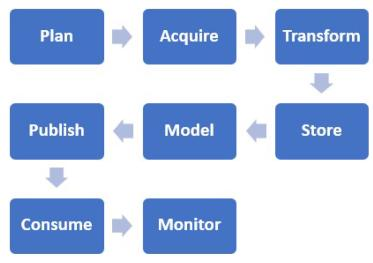
\includegraphics[scale=0.5]{images/dataops-workflow}
    \label{fig:dataops-workflow}
\end{figure}

Below are the key steps derived from a systematic literature review\cite{FANNOUCH2025100321}:

\subsubsection{Data Orchestration}
Data orchestration involves automating the flow of data from its source through various transformation steps to its final destination.
This helps reduce human error and makes the process more efficient.
It's also important to carefully manage how data moves from one stage to the next—for example,
from raw data to cleaned data and then to analysis-ready formats—so that everything flows in the correct order.

\subsubsection{Data Governance}
Good data governance means making sure the data is accurate and trustworthy.
This includes checking and cleaning the data, so it's consistent and correct.
It also means protecting the data through encryption and access controls,
and ensuring that all processes follow legal regulations such as GDPR.

\subsubsection{Continuous Integration and Deployment (CI/CD)}
CI/CD practices help teams work together smoothly by keeping track of changes in both code and data.
They also involve automatically testing pipelines to catch problems early,
which helps maintain quality and reliability as the system evolves.

\subsubsection{Monitoring and Observability}
Monitoring is about checking how the system is performing—measuring things like speed, error rates,
and resource usage.
Observability adds transparency by logging changes and tracking how data is accessed,
which helps with debugging and maintaining trust in the system.

\subsection{DataOps Integration with MLOps}\label{subsec:dataops-mlops-integration}

The integration of DataOps with MLOps creates a seamless workflow from raw data to deployed ML models.
This integration addresses several critical challenges\cite{ad-hoc-dataops}:
DataOps serves as the foundation for MLOps by ensuring robust and reliable data processes that support the entire machine learning lifecycle.
It enables effective data preparation by cleaning, transforming, and validating data before it enters ML pipelines.
Through feature engineering, DataOps helps convert raw data into meaningful inputs that improve model performance.
Data versioning is also a key component, allowing teams to track data lineage and ensure the reproducibility of machine learning experiments.
Additionally, data quality monitoring plays a vital role in detecting data drift or anomalies that could negatively impact model outcomes, ensuring models remain accurate and trustworthy over time.

According to\cite{dataops-mlops}, organizations that implement integrated DataOps and MLOps practices
realize significant advantages in
operational efficiency.

The evolution from ad hoc data analytics towards DataOps shows (fig:~\ref{fig:dataops-evo}) it follows the path to more automation
and is similar to the MLOps evolution we'll see later (fig:~\ref{fig:maturity}).
\begin{figure}[!htbp]
    \caption{DataOps Evolution\cite{ad-hoc-dataops}}
    \centering
    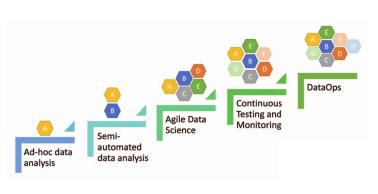
\includegraphics[scale=0.6]{images/dataops-evo}
    \label{fig:dataops-evo}
\end{figure}

